\chapter{Evaluation of the single policy algorithms.}

\section{Introduction.}
Last two chapters provided necessary background information, as well as, arguments for empirical evaluation of multi-objective reinforcement learning algorithms. This and all following chapters will be concentrating on an empirical analysis of different groups of algorithms. This chapter will focus on single policy algorithms. That is, algorithms which upon completion will produce an optimal value function for one policy. Two of the most common approaches are based on the well-established techniques from the multiobjective optimization: linear-weighted averages and lexicographic ordering (see Section \ref{sec:Selecting-a-solution-in-the-Pareto-Front} for explanation of both techniques).

It is impossible to say which approach is better, rather like two non-dominated policies, these techniques are not comparable. Both have strong and weak points and ultimately the decision which algorithm to use should be based on a problem at hand. This chapter will present empirical results of both approaches for a range of test problems. Each of the problems exhibits a property found in realistic domains which will significantly affect the performance an algorithm under consideration.

\subsection{Weighted Scalarization.}
Section \ref{sec:linear-temporal-difference-learning} documented how the linear-weighted averages algorithm was adopted in multi-objective reinforcement learning. Arguably the most seminal work in this direction was the linear-weighted averages implementation by Castelleti et al., (2002\nocite{castelletti2002reinforcement}), which is essentially a weighted scalarization of objective functions to reduce a multi-objective problem to a single objective one. 

Weighted scalarization allows an experimenter to locate a single point of the Pareto front. The located point depends on a set of preferences which was given to the algorithm. By gradually changing the preferences over objectives the algorithm can locate optimal value functions for different policies, thus approximating the Pareto front.

An experiment structure for this type of a single policy algorithm was given in Section \ref{sec:experiment-structure}. It is important to point out that a priori the experimenter does not know which preferences correspond to which policy and the experimenter will need to perform a number of test learning episodes to get an idea of a shape of a Pareto front for some MOMDP.

\subsection{Thresholded Lexicographic Ordering.}
Gabor, Kalmar and Szepesvari (1998)\nocite{gabor1998multi} implemented lexicographic ordering of objectives in their algorithm called thresholded lexicographic ordering (see Section \ref{sec:non-linear-temporal-difference-learning}). Lexicographic ordering of objectives relies on restricting all but one of the objectives to a certain threshold values thus allowing to use a maximization operator on the last unrestricted objective. This requires a domain knowledge which is not always practical to obtain, however, in many realistic domains it is possible to probe a problem with weighted scalarization to obtain a range of values for each of the objectives and use that knowledge to build a system of thresholds which will cover a Pareto front for the problem.
\begin{figure}[ht]
\centering
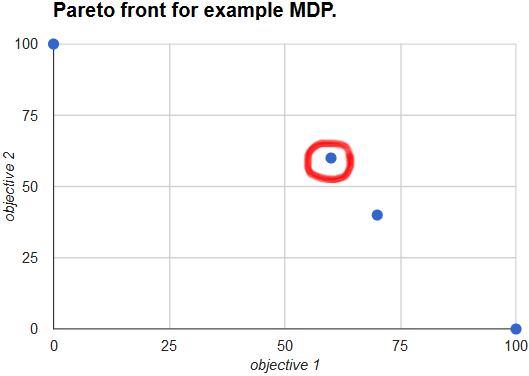
\includegraphics[scale=0.6]{exampleMDPOneMarkedPolicy.png}
\caption{Using the weighted scalarization will provide insights about points of a Pareto front for some problem. In this example the weighted scalarization identified one member of the Pareto front and obtained information can be used to specify thresholds for the thresholded lexicographic ordering algorithm. The blue dot which represents the policy with return [60,60] is marked with a red circle. The linear-scalarized single policy algorithm mentioned above will learn the Q-function for the policy associated with the marked blue dot, when given weight \{0.4,0.6\}}
\label{fig:how-tlo-works}
\end{figure}

To illustrate how weighted scalarization allows an experimenter to obtain the threshold values consider the Figure \ref{fig:how-tlo-works}. This is the example MOMDP with two objectives from Chapter two (see Section \ref{sec:experiment-structure}) with four non-dominated policies. An experimenter randomly chooses a set of weights $ \textbf{w} $ (for example let $ \textbf{w} = \{0.4,0.6\} $). This will make weighted scalarization to learn optimal value function for the policy with return [60,60] (marked with a red circle on the Figure \ref{fig:how-tlo-works}). After that the experimenter initializes the thresholded lexicographic ordering algorithm with the threshold of 60 for the first objective and starts the algorithm. The algorithm will try to maximize the second objective given that it satisfied the threshold for the first objective.

\section{Empirical Results.}

\subsection{Deep Sea Treasure.}
For problem specification see Section \ref{sec:deep-sea-treasure}.

Deep Sea Treasure is an interesting problem because of the fact that one of the objectives, treasure, is extrinsic and the second one, time, is intrinsic. In addition the Pareto front for this problem is globally concave. This structure of rewards is really suitable for showcasing advantages of TLO algorithm over WS.

Table \ref{tab:deep-sea-treasure} shows the results of WS and TLO runs on the Deep Sea Treasure. As was expected the WS algorithm was not able to find concave Pareto front members. Contrary to the WS, the TLO algorithm was able to locate concave Pareto front members. So the TLO was able to find extreme members of the Pareto front as well as intermediate, this leads to higher hypervolume values.

\begin{table}[t]
\centering
\def\arraystretch{1.5}
\begin{tabular}{|c|c|c|c|c|c|}
  \hline
  % after \\: \hline or \cline{col1-col2} \cline{col3-col4} ...
  & 10k & 20k & 30k & 40k & 50k \\
  \hline
  WS & 388 & 292 & 462 & 288 & 142 \\
  \hline
  TLO & 460 & 510 & 510 & 510 & 510 \\
  \hline
\end{tabular}
\caption{TLO and WS algorithms tested on Deap Sea Treasure. Reference point is (0,-20). Epsilon is 0.17, alpha is 0.9, gamma is 1.0. Step limit is 200 per episode.}
\label{tab:deep-sea-treasure}
\end{table}

\begin{figure}[ht]
\centering
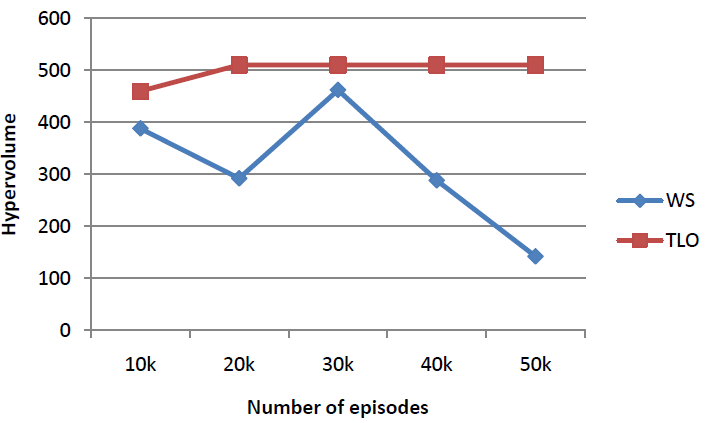
\includegraphics[scale=0.6]{DSTResults.png}
\caption{WS vs TLO tested on Deep Sea Treasure. Reference point is (0;-20). Epsilon is 0.17, alpha is 0.9, gamma is 1.0.}
\label{fig:ws-tlo-dst-results}
\end{figure}

\subsection{MO-PuddleWorld.}
For problem specification see Section \ref{sec:mo-puddleworld}.

The reward structure for MO-PuddleWorld has one intrinsic reward, namely the time penalty, which is -1 on all steps except goal state, when penalty is 0. The second reward, namely puddle penalty, is extrinsic. The MO-PuddleWorld test problem represents a state as a combination of two continuous variables: x position and y position. A 20 by 20 discretization was used in case of both the TLO and the WS algorithms. Tables \ref{tab:mo-puddleworld-1} and \ref{tab:mo-puddleworld-2} provide details of WS and TLO algorithms ran from 5 different starting positions. Fixed positions were used to remove the effects of noise due to random starting positions.

The results of the two algorithms are very similar. This can be explained by the nature of the problem itself. In the deep sea treasure problem the shape of the Pareto front provides a number of concave solutions and the TLO algorithm can converge to any point in that front, which increases the hypervolume. Contrary, the MO-PuddleWorld's Pareto front from most of the starting points is primarily convex in shape, and when concave solutions are available, a number of those solutions is very small and they contribute only slightly to the overall hypervolume attainable. So the TLO algorithm never receives a chance to showcase its benefits over the WS algorithm.

\begin{table}[t]
\centering
\def\arraystretch{1.5}
\begin{tabular}{|c|c|c|c|c|c|}
  \hline
  % after \\: \hline or \cline{col1-col2} \cline{col3-col4} ...
  & (0.25;0.6) & (0.35;0.55) & (0.3;0.55) & (0.3;0.7) & (0.2;0.7) \\
  \hline
  0 & 1084 & 988 & 99 & 99 & 99 \\
  \hline
  500 & 7998 & 8084 & 7984 & 8287 & 8087 \\
  \hline
  1000 & 7998 & 8084 & 7998 & 8297 & 8098 \\
  \hline
\end{tabular}
\caption{WS algorithm tested on MO-PuddleWorld problem with 5 different starting positions. Reference point is (-100,-100). Epsion is 0.15, alpha is 0.9, gamma is 1.0. Step limit is 100 steps per episode.}
\label{tab:mo-puddleworld-1}
\end{table}

\begin{table}[t]
\centering
\def\arraystretch{1.5}
\begin{tabular}{|c|c|c|c|c|c|}
  \hline
  % after \\: \hline or \cline{col1-col2} \cline{col3-col4} ...
  & (0.25;0.6) & (0.35;0.55) & (0.3;0.55) & (0.3;0.7) & (0.2;0.7) \\
  \hline
  0 & 99 & 100 & 99 & 99 & 99 \\
  \hline
  500 & 7984 & 8083 & 7984 & 8287 & 8087 \\
  \hline
  1000 & 7984 & 8083 & 7984 & 8287 & 8087 \\
  \hline
\end{tabular}
\caption{TLO algorithm tested on MO-PuddleWorld problem with 5 different starting positions. Reference point is (-100,-100). Epsion is 0.15, alpha is 0.9, gamma is 1.0. Step limit is 100 steps per episode.}
\label{tab:mo-puddleworld-2}
\end{table}

\subsection{MO-MountainCar.}
For problem specification see Section \ref{sec:mo-mountain-car}.

The reward structure for mountain car problem consists of 3 intrinsic rewards. The first is a penalty of -1 applied each time step, the second is a penalty of -1 applied at every backward acceleration and the third one is a penalty of -1 applied at every forward acceleration. The MO-MountainCar test problem represents a state as a combination of two continuous variables: a position and a velocity. A 170(position) by 140(velocity) discretization was used in case of both the TLO and the WS algorithms.

\begin{table}[t]
\centering
\def\arraystretch{1.5}
\begin{tabular}{|c|c|c|c|c|c|}
  \hline
  % after \\: \hline or \cline{col1-col2} \cline{col3-col4} ...
  & 5k & 15k & 25k & 35k & 40k \\
  \hline
  1 & 6,065,247 & 11,819,348 & 15,175,815 & 15,322,349 & 15,322,597 \\
  \hline
  2 & 5,357,800 & 10,926,832 & 15,137,425 & 15,417,314 & 15,416,766 \\
  \hline
  3 & 5,785,239 & 11,629,691 & 14,865,468 & 15,302,728 & 15,303,667 \\
  \hline
  4 & 6,786,636 & 10,713,965 & 15,068,736 & 15,442,287 & 15,443,135 \\
  \hline
  5 & 7,870,923 & 10,963,501 & 14,941,997 & 15,270,617 & 15,326,463 \\
  \hline
  AVG & 6,373,169 & 11,210,667 & 15,037,888 & 15,351,059 & 15,362,525 \\
  \hline      
\end{tabular}
\caption{WS algorithm results on MO-MountainCar problem over 5 runs. Starting position is always fixed and is -0.5. Reference point is (-300;-300;-300). Epsilon is 0.0, alpha is 0.9, gamma is 1.0.}
\label{tab:mo-mountaincar-1}
\end{table}

Tables \ref{tab:mo-mountaincar-1} and \ref{tab:mo-mountaincar-2} show results of the WS and the TLO algorithms. As you can see the WS algorithm outperformed the TLO algorithm. This can be explained by the intrinsic rewards. The linear combination of objectives used to perform action-selection in the WS algorithm is compatible with both intrinsic and extrinsic rewards. However TLO’s non-linear action selection mechanism performs poorly when thresholding is applied to intrinsic rewards, as it fails to account for the rewards already received earlier in the episode. Thus TLO was heavily impacted by the intrinsic rewards, which resulted in poor figures of hypervolume. This observation is compatible with the preliminary results reported in Vamplew et al. (2011)\nocite{vamplew2011empirical}, who noted TLO performs poorly on the Deep Sea Treasure task if the ordering of the objectives is changed such that the intrinsic reward is being thresholded.

\begin{table}[t]
\centering
\def\arraystretch{1.5}
\begin{tabular}{|c|c|c|c|c|c|}
  \hline
  % after \\: \hline or \cline{col1-col2} \cline{col3-col4} ...
  & 5k & 15k & 25k & 35k & 40k \\
  \hline
  1 & 85,349 & 9,315,462 & 11,798,739 & 11,925,448 & 11,942,691 \\
  \hline
  2 & 85,591 & 9,970,806 & 12,590,952 & 12,883,731 & 12,879,446 \\
  \hline
  3 & 85,528 & 8,483,264 & 12,282,405 & 12,386,070 & 12,465,344 \\
  \hline
  4 & 85,460 & 10,951,818 & 12,525,832 & 12,549,660 & 12,549,715 \\
  \hline
  5 & 87,309 & 9,206,131 & 12,509,929 & 12,617,007 & 12,623,177 \\
  \hline
  AVG & 85,847 & 9,585,496 & 12,341,571 & 12,472,383 & 12,492,074 \\
  \hline
\end{tabular}
\caption{TLO algorithm results on MO-MountainCar problem over 5 runs. Starting position is always fixed and is -0.5. Reference point is (-300;-300;-300). Epsilon is 0.0, alpha is 0.9, gamma is 1.0.}
\label{tab:mo-mountaincar-2}
\end{table}

\begin{figure}[ht]
\centering
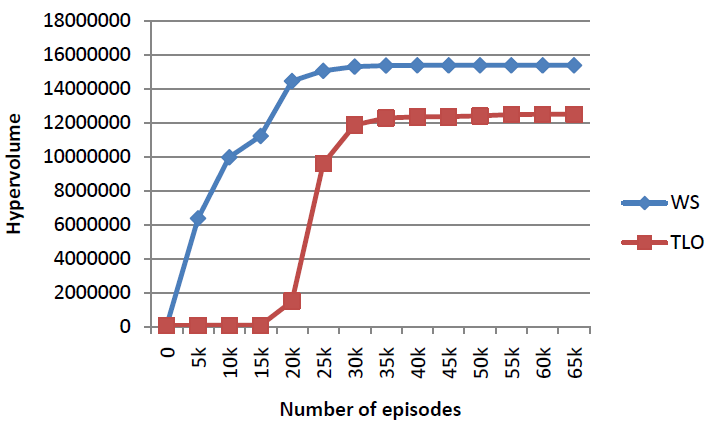
\includegraphics[scale=0.6]{MCResults.png}
\caption{WS vs TLO hypervolume growth on MO-MountainCar problem. Starting position is always fixed and is -0.5. Reference point is (-300;-300;-300). Epsilon is 0.0, alpha is 0.9, gamma is 1.0.}
\label{fig:ws-tlo-mc-results}
\end{figure}

\section{Conclusion.}
Three different problems were presented. Deep Sea Treasure and MO-PuddleWorld has similar reward structure. In that one of the objectives is extrinsic and the other one is intrinsic. Meanwhile the MO-MountainCar has all of its objectives being intrinsic.

Deep Sea Treasure has a number of concavities in Pareto front. The TLO algorithm clearly benefited from its ability to locate those concavities. The WS algorithm doesn’t have this ability and this leads to a situation where the WS algorithm was dominated by the TLO algorithm. The MO-PuddleWorld’s reward structure is similar to the one of Deep Sea Treasure but this doesn’t lead to similar dominance. This can be explained by the nature of the MO-PuddleWorld problem. The MO-PuddleWorld’s Pareto front from any starting position has concavities, but the number of those concavities is not comparable to Deep Sea Treasure and for some starting positions there are no concavities at all. This lead to a situation where the TLO algorithm was not able to benefit from its main strength and showed similar results as the WS algorithm. The MO-MountainCar benchmark highlighted the dominance of the WS algorithm over the TLO in problems with intrinsic rewards.

In summary this chapter demonstrates the importance of empirical studies on benchmark problems with known characteristics in establishing the conditions under which different MORL algorithms will work effectively. Clearly the TLO algorithm can only be used reliably on problems with no more than one intrinsic reward. However where the reward structure of an environment does meet this criteria, TLO is likely to outperform WS due to its capacity to discover policies which lie in concave regions of the Pareto front which cannot be found by the WS algorithm.
